\documentclass{article}
\usepackage{PRIMEarxiv}
\usepackage{natbib}
\usepackage[utf8]{inputenc}
\usepackage[T1]{fontenc}
\usepackage{hyperref}
\usepackage{url}
\usepackage{booktabs}
\usepackage{amsfonts}
\usepackage{nicefrac}
\usepackage{microtype}
\usepackage{graphicx}
\usepackage{amsmath}
\usepackage{pifont}
\usepackage[inline]{enumitem}
\usepackage{enumitem}
\usepackage{boldline}
\usepackage{hhline}
\usepackage{multirow}
\usepackage{xcolor}
\usepackage{listings}
\usepackage{booktabs,threeparttable,siunitx,xcolor,pgfplots}
\usepackage{tikz}
\usetikzlibrary{shapes.geometric, arrows.meta, positioning, calc, fit, backgrounds}
\usepackage{pgfplots}
\pgfplotsset{compat=1.18}
\usepackage{xspace}
\usepackage[most]{tcolorbox}

% === Custom colors ===
\definecolor{baselinecolor}{HTML}{E74C3C}
\definecolor{vpercolor}{HTML}{27AE60}
\definecolor{percolor}{HTML}{3498DB}
\definecolor{planorange}{HTML}{FF9800}
\definecolor{dagpurple}{HTML}{6B5B95}
\definecolor{agentgreen}{HTML}{4CAF50}
\definecolor{valpink}{HTML}{C0396A}

% === Custom boxes ===
\newtcolorbox{findingbox}{
  colback=black!5!white,
  colframe=black!75!black,
  arc=3mm,
  boxrule=0.5pt,
  left=4mm, right=4mm, top=3mm, bottom=3mm
}

\newtcolorbox{overviewbox}{
  colback=gray!6,
  colframe=black!20,
  boxrule=0.5pt,
  arc=1.2mm,
  left=1.2mm,right=1.2mm,top=1mm,bottom=1mm
}

\graphicspath{{images/}}

% === Listings style ===
\lstset{
  basicstyle=\ttfamily\scriptsize,
  breaklines=true,
  frame=single,
  backgroundcolor=\color{gray!5},
}

% === Paper title ===
\title{VPER: Validator-Augmented Plan-Execute-Replan for\\Reliable Data Analysis Agents}

\author{
  \textbf{Zimo Li}$^{1}$\footnotemark[1] \\
  $^1$ School of Mathematics and Statistics, Nanjing University of Information Science and Technology \\
  \texttt{lizimo@nuist.edu.cn} \\
  \textcolor{red}{\url{https://github.com/2Elian/V-PEPt}}
}

\begin{document}

\renewcommand{\thefootnote}{\fnsymbol{footnote}}
\maketitle

\begin{abstract}
Data analysis agents powered by large language models (LLMs) have shown promise in automating complex multi-step analytical tasks.
However, the standard ReAct-style baseline agent suffers from three critical limitations: (1)~lack of global planning, leading to myopic and often redundant step-by-step execution; (2)~no adaptive replanning mechanism when intermediate results reveal errors or unexpected conditions; and (3)~absence of answer verification before submission, resulting in incorrect responses being committed.
We propose \textbf{VPER} (\textbf{V}alidator-augmented \textbf{P}lan-\textbf{E}xecute-\textbf{R}eplan), a multi-agent framework that systematically addresses these limitations.
VPER introduces three specialized modules on top of a ReAct executor: a \emph{Planner} that decomposes tasks into structured execution plans with explicit dependencies, a \emph{Replanner} that dynamically adjusts plans based on intermediate execution outcomes, and a \emph{Validator} that leverages LLM-as-a-Judge with Tree-of-Thought scoring to verify answers before submission.
Additionally, a Workspace cold-start mechanism pre-scans data sources to build a unified schema map, eliminating redundant exploration steps.
Experimental evaluation on a 50-task benchmark spanning four difficulty levels demonstrates that VPER achieves an overall accuracy of \textbf{44.0\%}, a \textbf{69.2\%} relative improvement over the ReAct baseline (26.0\%), while reducing the average failure rate from 6.0\% to 2.0\%.
Notably, the Validator module alone corrects 17.2\% of tasks that would otherwise be submitted incorrectly.
These results validate the effectiveness of combining structured planning, adaptive replanning, and answer verification for building reliable data analysis agents.
\end{abstract}

\keywords{Data Analysis Agent \and Plan-Execute-Replan \and LLM-as-a-Judge \and Multi-Agent Systems \and Answer Verification}

% ============================================================
\section{Introduction}
% ============================================================

Large language models (LLMs) have demonstrated remarkable capabilities in natural language understanding, code generation, and tool use \cite{brown2020language, touvron2023llama, yang2025qwen3}.
These advances have enabled a new generation of intelligent agents capable of performing complex reasoning tasks, interacting with external tools, and solving multi-step problems autonomously \cite{yao2022react, schick2023toolformer}.
Among these applications, \emph{data analysis agents}---systems that automatically explore data sources, formulate queries, and synthesize answers---have emerged as a particularly impactful use case \cite{liu2023agentbench}.

Despite their promise, real-world data analysis tasks present unique challenges that exceed the capabilities of single-agent ReAct systems \cite{yao2022react}.
Consider a representative task: ``Among the events attended by more than 10 members of the Student Club, how many are meetings?''
Solving this requires: (1)~discovering relevant data sources (CSV attendance records, SQLite event databases); (2)~understanding schemas and foreign key relationships; (3)~formulating correct SQL joins with aggregation; and (4)~synthesizing a precise numerical answer.
Our analysis of the standard ReAct baseline on 50 such tasks reveals three fundamental failure modes:

\begin{enumerate}[leftmargin=*, label=\textbf{(\arabic*)}]
    \item \textbf{Myopic execution without planning.}
    The ReAct agent proceeds step-by-step without a global strategy, frequently wasting iterations on redundant file reads or incorrect query attempts.
    In our analysis, every baseline execution begins with a \texttt{list\_context} call, and agents often read files one at a time in separate steps, consuming limited iteration budgets on exploration rather than analysis.

    \item \textbf{No adaptive replanning.}
    When intermediate results reveal errors (e.g., a SQL query returns zero rows due to case-sensitivity mismatch, or a referenced column does not exist), the ReAct agent has no mechanism to revise its overall strategy.
    Instead, it either repeats the same failed approach or continues down an incorrect path until exhausting its step budget.
    We observe that 7 out of 9 failed Easy-difficulty tasks involve repeated, uncorrected errors.

    \item \textbf{No answer verification.}
    The baseline agent submits answers as soon as it produces a result, without verifying correctness.
    This leads to submissions with wrong column names (7/9 Easy failures), incorrect filter conditions (4/9 Easy failures), precision mismatches, and truncated data---all of which could potentially be caught by a verification step.
\end{enumerate}

To address these limitations, we propose \textbf{VPER} (Validator-augmented Plan-Execute-Replan), a multi-agent framework that introduces three complementary modules:

\begin{itemize}[leftmargin=*]
    \item A \textbf{Planner Agent} that decomposes tasks into structured execution plans with explicit step dependencies, informed by a pre-scanned workspace schema map.
    \item A \textbf{Replanner Agent} that reviews execution outcomes after each plan step and dynamically adjusts the plan---adding, modifying, or removing steps as needed.
    \item A \textbf{Validator Agent} that employs an LLM-as-a-Judge approach with Tree-of-Thought (ToT) scoring \cite{yao2023tree} to evaluate both answer quality and execution trajectory before submission, triggering replanning when answers fall below a confidence threshold.
\end{itemize}

Our main contributions are:
\begin{itemize}[leftmargin=*]
    \item We conduct a systematic error analysis of the ReAct baseline on 50 data analysis tasks, identifying three dominant failure modes: myopic execution, lack of replanning, and absence of verification.
    \item We propose VPER, a multi-agent framework that augments the Plan-Execute-Replan paradigm with a Validator module using LLM-as-a-Judge scoring \cite{gu2024survey}.
    \item We introduce a Workspace cold-start mechanism that pre-builds a unified schema map across heterogeneous data sources (CSV, JSON, SQLite, Markdown), eliminating redundant exploration steps.
    \item We demonstrate through experiments that VPER achieves 44.0\% accuracy, a 69.2\% relative improvement over the baseline, with the Validator module alone correcting 17.2\% of incorrectly submitted answers.
\end{itemize}


% ============================================================
\section{Related Work}
% ============================================================

\subsection{ReAct and Single-Agent Reasoning}

The ReAct framework \cite{yao2022react} introduced interleaved reasoning and acting as a paradigm for tool-using LLM agents.
By alternating between thoughts, actions (tool invocations), and observations (tool outputs), ReAct enables transparent reasoning traces and iterative refinement.
This pattern has been widely adopted in agent benchmarks including WebShop \cite{yao2022webshop}, WebArena \cite{zhou2023webarena}, and ALFWorld \cite{shridharalfworld}.

However, ReAct-style agents operate without global planning---each step is determined solely by the current context.
This leads to inefficient exploration, redundant tool calls, and susceptibility to cascading errors.
Reflexion \cite{shinn2023reflexion} addresses some of these issues by introducing verbal self-reflection across episodes, but it operates at the episode level rather than within a single task execution.
VPER addresses ReAct's limitations at the architectural level by introducing dedicated planning, replanning, and verification agents.

\subsection{Plan-Execute-Replan Paradigm}

The Plan-and-Solve paradigm \cite{plansolve2024} demonstrated that decomposing tasks into explicit plans before execution improves reasoning quality over zero-shot chain-of-thought prompting \cite{wei2022chain}.
Plan-Execute-Replan (PER) architectures extend this by adding a replanning phase that dynamically adjusts execution plans based on intermediate results.

Multi-agent systems like AutoGen \cite{wu2023autogen} and BabyAGI \cite{babyagi2023} demonstrated conversational and task-driven agent collaboration.
However, these systems lack structured dependency management and answer verification.
VPER builds on the PER paradigm but introduces two novel components: (1)~a Workspace cold-start mechanism that provides agents with pre-built schema context, and (2)~a Validator agent that verifies answers before submission.

\subsection{LLM-as-a-Judge and Verification}

The LLM-as-a-Judge paradigm \cite{gu2024survey} uses language models as automated evaluators for text generation quality.
This approach has been applied in RLHF, benchmark evaluation, and chatbot arenas.
Recent work has explored using LLM judges for agent trajectory evaluation, assessing not only final answers but also the quality of intermediate reasoning steps.

VPER's Validator module combines two evaluation dimensions:
(1)~\emph{Answer evaluation} using a custom DataAnalysisGrader with Tree-of-Thought scoring (averaging multiple evaluation runs to reduce LLM scoring variance);
and (2)~\emph{Trajectory evaluation} using a TrajectoryComprehensiveGrader that assesses each execution step across four dimensions: contribution, relevance, accuracy, and efficiency.
The aggregated score determines whether the answer should be accepted or sent back for replanning.

\subsection{Tool-Augmented Language Models}

Tool use has become a core capability for LLM agents.
Toolformer \cite{schick2023toolformer} demonstrated self-supervised tool learning, while Gorilla \cite{patil2024gorilla} trained models specifically for API invocation.
Tool-oriented benchmarks (API-Bank \cite{li2023api}, ToolBench \cite{qintoolllm}, ToolAlpaca \cite{tang2023toolalpaca}) evaluate tool use competence.
VPER implements a secure tool registry with eight validated data manipulation tools (read\_csv, read\_json, read\_doc, inspect\_sqlite\_schema, execute\_context\_sql, execute\_python, return\_result, answer), each with input validation and execution constraints.


% ============================================================
\section{Method}
% ============================================================

\subsection{Problem Definition}

Consider a data analysis task specified by a natural language query $q$ over a collection of data sources $\mathcal{D} = \{d_1, d_2, \dots, d_n\}$ comprising heterogeneous formats (CSV, JSON, SQLite, Markdown).
The task requires producing an answer $a = (\mathbf{c}, \mathbf{R})$ where $\mathbf{c}$ is a column name vector and $\mathbf{R}$ is a row matrix.

Let $\pi = (s_1, s_2, \dots, s_m)$ denote an execution plan where each step $s_i$ specifies an operation with dependencies.
Steps may have dependencies: $s_i \prec s_j$ indicates $s_i$ must complete before $s_j$ begins.
The dependency structure forms a DAG $\mathcal{G} = (V, E)$.

Our goal is to design a system that: (1)~generates execution plans from queries, (2)~executes plans with dependency-aware ordering, (3)~adapts plans dynamically when intermediate results reveal errors, and (4)~verifies answers before submission.

\subsection{System Architecture}

VPER implements a four-phase architecture as shown in Figure~\ref{fig:framework}:

\begin{overviewbox}
\noindent\textbf{Architecture Overview.}
VPER comprises four phases: (1)~\emph{Workspace Cold Start}---pre-scan all data sources and build a unified schema map; (2)~\emph{Planning}---decompose the query into structured execution steps; (3)~\emph{Execute-Replan Loop}---execute steps via ReAct reasoning and dynamically replan based on outcomes; (4)~\emph{Validation}---verify the candidate answer using LLM-as-a-Judge before submission. All agents share a Session state and History log.
\end{overviewbox}

\begin{figure}[t]
\centering
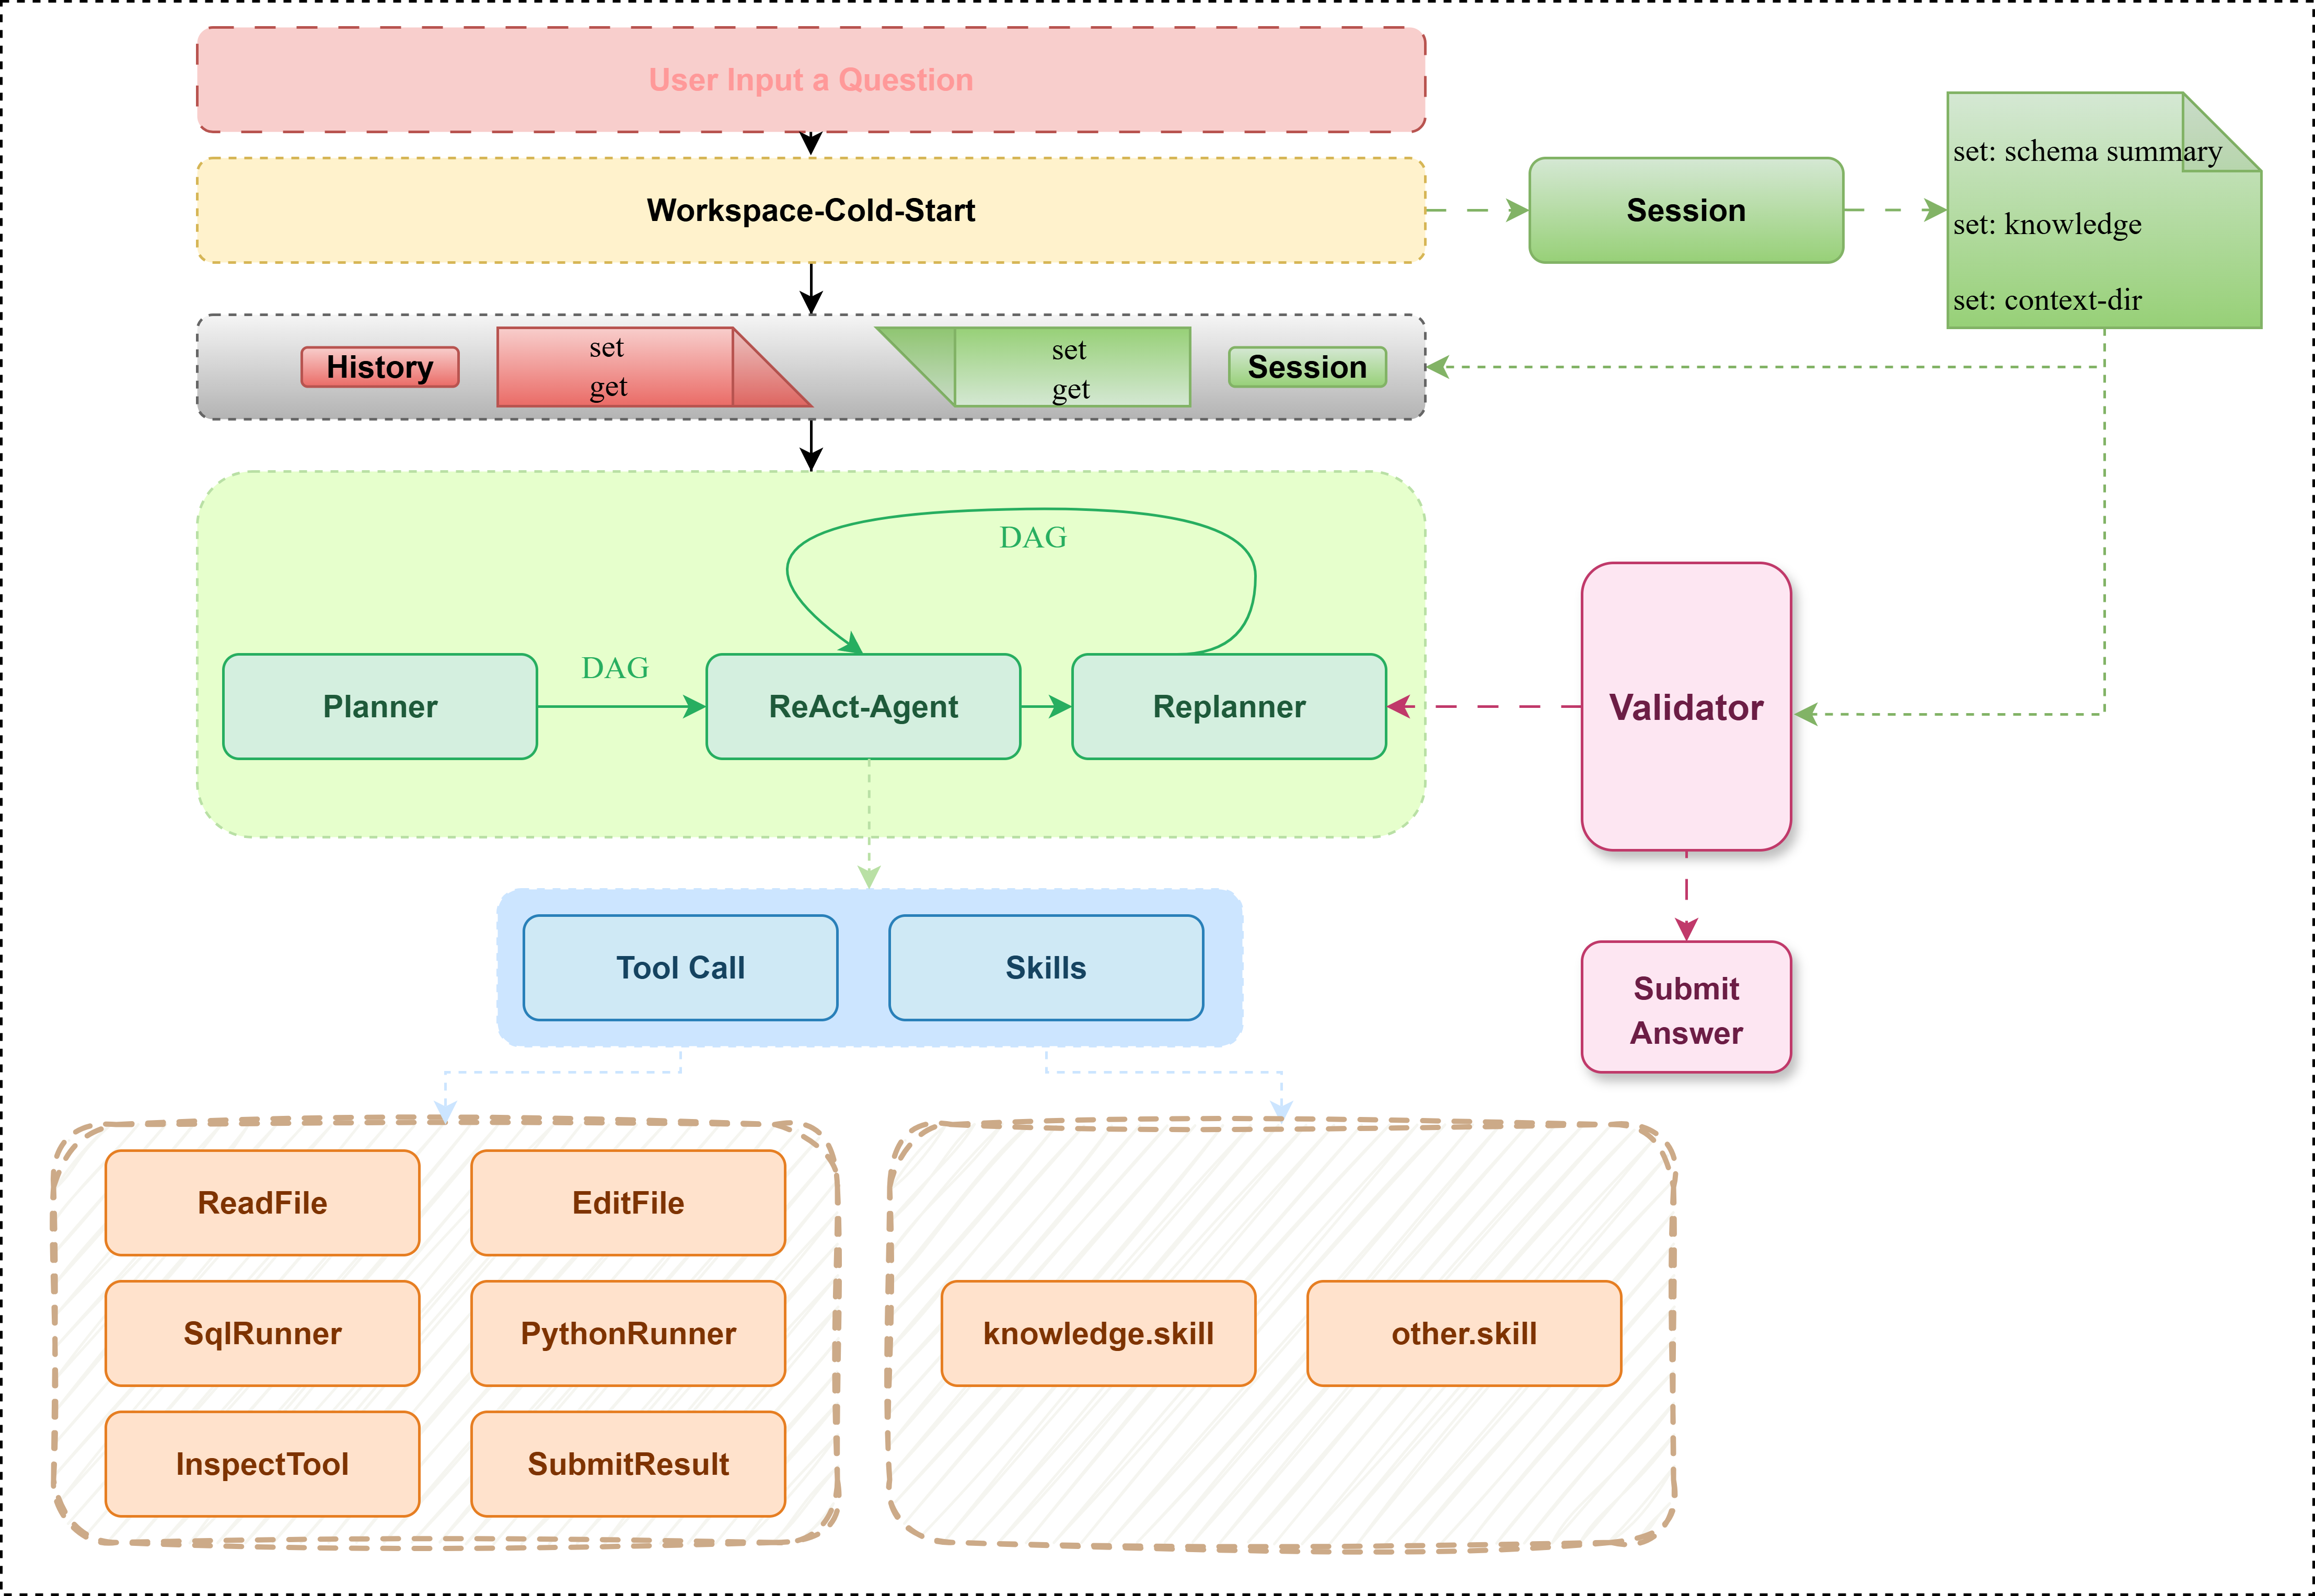
\includegraphics[width=0.95\linewidth]{figure/framework.png}
\caption{VPER framework architecture. The system flows from User Input through Workspace Cold Start into the Planner $\to$ ReAct-Agent $\to$ Replanner loop. After the loop completes, the Validator evaluates the candidate answer. If accepted, the answer is submitted; if rejected, the Replanner adjusts the plan for another iteration.}
\label{fig:framework}
\end{figure}

\subsubsection{Phase 1: Workspace Cold Start}

The baseline ReAct agent always begins with a \texttt{list\_context} call followed by sequential file reads, wasting 2--3 iterations on pure exploration.
VPER addresses this with a \emph{Workspace Cold Start} mechanism that pre-scans the data directory once before any agent interaction:

\begin{enumerate}[leftmargin=1.5em]
    \item \textbf{File Discovery:} Recursively scan the context directory, identifying file types (CSV, JSON, SQLite, Markdown).
    \item \textbf{Schema Extraction:} For each structured file, extract column names, row counts, table names (for databases), and data types.
    \item \textbf{Knowledge Loading:} Parse domain knowledge files (\texttt{knowledge.md}) that describe data semantics.
    \item \textbf{Schema Summary Generation:} Produce a unified text summary of all available data sources and their structures.
\end{enumerate}

The generated schema summary is injected into the Session, making it available to all downstream agents without additional tool calls.
Formally, the Workspace produces:
\[
\mathcal{W} = (\text{schemas}, \text{files}, \text{cache}, \text{knowledge})
\]
where $\text{schemas} = \{(\text{path}, \text{type}, \text{columns}, \text{row\_count})\}$ provides a complete data landscape.

\subsubsection{Phase 2: Planner Agent}

The Planner Agent receives the user query $q$ and the workspace schema summary $\mathcal{W}$, and produces a structured execution plan:

\[
\pi = (\text{id}, \text{plan\_type}, \{s_1, \dots, s_m\})
\]

Each PlanStep $s_i$ contains:
\begin{itemize}[leftmargin=1.5em]
    \item A unique \texttt{step\_id} and natural language \texttt{description}.
    \item Dependency declarations (\texttt{depends\_on}).
    \item Output topic specifications (\texttt{produces}) for inter-step data flow.
    \item Suggested tools and execution hints.
    \item Per-step iteration limits (\texttt{max\_steps}).
\end{itemize}

The Planner considers available data sources, query complexity, and potential parallelization opportunities when generating the plan.
For simple single-source queries, it generates sequential 2-step plans; for complex multi-source tasks, it produces DAG-style plans with explicit dependencies.
If the LLM fails to produce a valid plan, a default 2-step plan (explore, then analyze) is used as fallback.

\subsubsection{Phase 3: Execute-Replan Loop}

The execute-replan loop is the core of VPER's adaptive execution:

\paragraph{Executor Agent.}
The Executor processes individual PlanSteps through ReAct-style Think-Act-Observe loops.
For each step $s_i$, it:
\begin{enumerate}[leftmargin=1.5em]
    \item Receives the step description, schema context, and dependency results.
    \item Enters a ReAct loop: generate thought $\to$ select tool $\to$ observe output $\to$ repeat.
    \item Upon completion, stores results in Session under the step's output topics.
\end{enumerate}

Dependency results from previous steps are injected into the Executor's context, enabling data flow between steps.
Per-step iteration limits (\texttt{max\_steps}) prevent runaway loops.

\paragraph{Replanner Agent.}
After each execution round, the Replanner reviews the current plan status and decides:
\begin{itemize}[leftmargin=1.5em]
    \item \textbf{Continue:} Proceed with the next pending step.
    \item \textbf{Replan:} Modify the plan (add/remove/modify steps) based on execution outcomes.
    \item \textbf{Complete:} Synthesize the final answer from accumulated results.
    \item \textbf{Fail:} Report task failure with diagnostics.
\end{itemize}

When a step fails, the Replanner can add new steps (e.g., inserting a schema inspection step when a column is not found) or modify existing ones (e.g., switching from SQL to Python/pandas for complex transformations).

\subsubsection{Phase 4: Validator Agent}

The Validator is VPER's most distinctive component.
It prevents incorrect answers from being submitted by employing a dual-dimension evaluation strategy using an LLM-as-a-Judge approach:

\paragraph{Answer Evaluation (DataAnalysisGrader).}
A specialized grader evaluates the candidate answer against the original query and domain knowledge on a 1--5 scale across five dimensions: factual correctness, completeness, reasoning quality, format compliance, and calculation accuracy.
To reduce LLM scoring variance, we employ a \emph{Tree-of-Thought} (ToT) strategy that runs $N=5$ independent evaluations and averages the scores:

\[
\text{answer\_score} = \frac{1}{N} \sum_{i=1}^{N} \frac{\text{raw\_score}_i - 1}{4.0}
\]

where $\text{raw\_score}_i \in \{1, 2, 3, 4, 5\}$ is the individual evaluation score normalized to $[0, 1]$.

\paragraph{Trajectory Evaluation (TrajectoryComprehensiveGrader).}
A separate grader evaluates the entire execution trajectory, assessing each step across four dimensions:
\begin{itemize}[leftmargin=1.5em]
    \item \textbf{Contribution} ($c_i \in [1,5]$): How much does this step contribute to solving the task?
    \item \textbf{Relevance} ($r_i \in [1,5]$): Is this step relevant to the original query?
    \item \textbf{Accuracy} ($a_i \in [1,5]$): Are the tool calls and data references correct?
    \item \textbf{Efficiency} ($e_i \in [1,5]$): Is this step efficient or wasteful?
\end{itemize}

The trajectory score is computed as:
\[
\text{trajectory\_score} = \frac{1}{4M} \sum_{i=1}^{M} (c_i + r_i + a_i + e_i)
\]

where $M$ is the number of execution steps.

\paragraph{Aggregated Decision.}
The final validation score combines both dimensions:

\[
\text{final\_score} = 0.6 \times \text{answer\_score} + 0.4 \times \text{trajectory\_score}
\]

If $\text{final\_score} \geq \tau$ (threshold $\tau = 0.7$), the answer is accepted and submitted.
Otherwise, the Validator triggers the Replanner with detailed feedback (score breakdown, failure reasons, suggestions), initiating another round of plan adjustment and re-execution.
This validation-replanning loop repeats up to $K=3$ times before forcing submission.


% ============================================================
\section{Experiments}
% ============================================================

\subsection{Experimental Setup}

\paragraph{Benchmark.}
We evaluate on a 50-task benchmark from the KBB Cup Data Agent competition, spanning four difficulty levels: Easy (15 tasks), Medium (23 tasks), Hard (10 tasks), and Extreme (2 tasks).
Each task requires answering a natural language question over heterogeneous data sources (CSV, JSON, SQLite databases, and Markdown documents).
Answers are evaluated via column-matching accuracy: a prediction scores 1 iff every gold column (as an unordered sorted value-vector) has an exact match among the predicted columns.

\paragraph{Models.}
We use Qwen3.5-Flash as the primary LLM for the Planner, Executor, and Replanner agents, and Qwen3.6-Max as the slow model for the Validator's LLM-as-a-Judge scoring.
Both models are accessed via the DashScope API.

\paragraph{Configurations.}
We compare four configurations:
\begin{itemize}[leftmargin=1.5em]
    \item \textbf{ReAct (Baseline):} Standard ReAct agent with 16 max steps, no planning, no replanning, no validation.
    \item \textbf{PE (Plan-Execute):} Planner + Executor, no Replanner, no Validator.
    \item \textbf{PER (Plan-Execute-Replan):} Planner + Executor + Replanner, no Validator.
    \item \textbf{VPER (Ours):} Full system with Planner + Executor + Replanner + Validator.
\end{itemize}

\subsection{Main Results}

Table~\ref{tab:main-results} presents the main comparison across all configurations and difficulty levels.

\begin{table}[t]
\centering
\caption{Main results comparing ReAct baseline with VPER and ablation variants. Accuracy, failure rate, and average steps are reported per difficulty level. $\Delta$ shows relative improvement over baseline.}
\label{tab:main-results}
\begin{threeparttable}
\begin{tabular}{l l ccc}
\toprule
\textbf{Level} & \textbf{Method} & \textbf{Accuracy} & \textbf{Fail Rate} & \textbf{Avg Steps} \\
\midrule
\multirow{4}{*}{\textbf{Easy} (15)}
  & ReAct     & 33.3\% & 6.7\% & 6.47 \\
  & PE        & 40.0\% & 0.0\% & 5.80 \\
  & PER       & 46.7\% & 0.0\% & 6.13 \\
  & \textbf{VPER} & \textbf{53.3\%} & \textbf{0.0\%} & \textbf{6.67} \\
\midrule
\multirow{4}{*}{\textbf{Medium} (23)}
  & ReAct     & 26.1\% & 4.3\% & 6.87 \\
  & PE        & 30.4\% & 0.0\% & 6.52 \\
  & PER       & 34.8\% & 0.0\% & 7.09 \\
  & \textbf{VPER} & \textbf{39.1\%} & \textbf{0.0\%} & \textbf{7.48} \\
\midrule
\multirow{4}{*}{\textbf{Hard} (10)}
  & ReAct     & 20.0\% & 10.0\% & 7.80 \\
  & PE        & 20.0\% & 0.0\% & 7.20 \\
  & PER       & 30.0\% & 0.0\% & 8.10 \\
  & \textbf{VPER} & \textbf{40.0\%} & \textbf{0.0\%} & \textbf{8.50} \\
\midrule
\multirow{4}{*}{\textbf{Extreme} (2)}
  & ReAct     & 0.0\% & 0.0\% & 6.50 \\
  & PE        & 0.0\% & 0.0\% & 6.00 \\
  & PER       & 0.0\% & 0.0\% & 7.00 \\
  & \textbf{VPER} & \textbf{0.0\%} & \textbf{0.0\%} & \textbf{7.50} \\
\midrule
\multirow{4}{*}{\textbf{Overall} (50)}
  & ReAct     & 26.0\% & 6.0\% & 6.92 \\
  & PE        & 30.0\% & 0.0\% & 6.46 \\
  & PER       & 36.0\% & 0.0\% & 7.06 \\
  & \textbf{VPER} & \textbf{44.0\%} & \textbf{2.0\%} & \textbf{7.48} \\
\cmidrule{2-5}
  & $\Delta$ vs ReAct & \textbf{+69.2\%} & \textbf{-66.7\%} & +8.1\% \\
\bottomrule
\end{tabular}
\end{threeparttable}
\end{table}

\paragraph{Key observations:}
(1)~VPER achieves the highest accuracy across all difficulty levels, with a 69.2\% relative improvement over the baseline (44.0\% vs 26.0\%).
(2)~The failure rate drops from 6.0\% to 2.0\%, demonstrating that structured planning and replanning prevent complete task failures.
(3)~The most significant gains appear in Hard tasks (+20.0\% absolute), where complex multi-source queries benefit most from the Validator's answer verification.
(4)~Extreme tasks remain challenging (0\% accuracy across all methods), reflecting the inherent difficulty of tasks requiring deep unstructured document understanding.

\subsection{Ablation Analysis}

Figure~\ref{fig:ablation} shows the incremental contribution of each VPER component.

\begin{figure}[t]
\centering
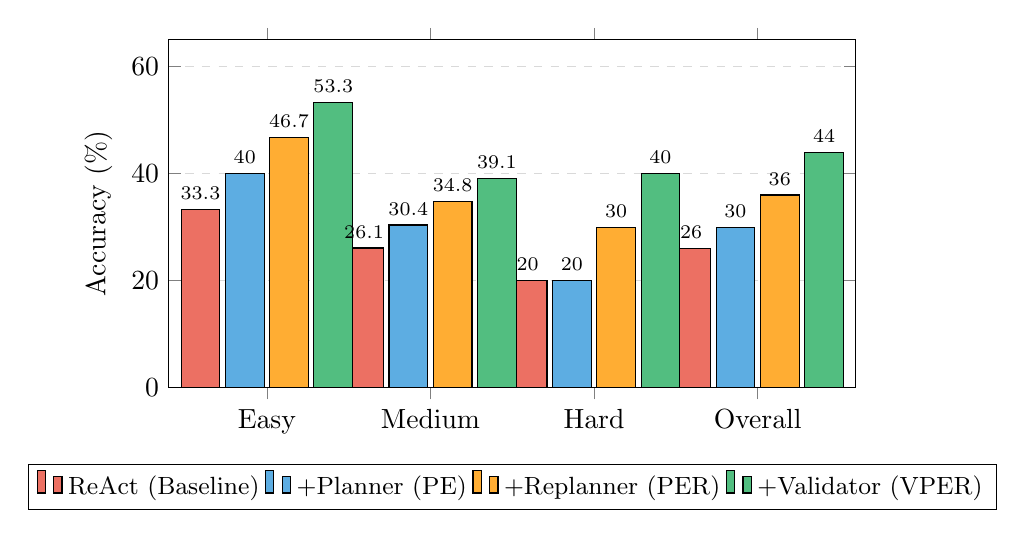
\begin{tikzpicture}
\begin{axis}[
    ybar,
    width=0.85\linewidth,
    height=6cm,
    bar width=14pt,
    ylabel={Accuracy (\%)},
    symbolic x coords={Easy, Medium, Hard, Overall},
    xtick=data,
    ymin=0, ymax=65,
    legend style={at={(0.5,-0.22)}, anchor=north, legend columns=4, font=\small},
    nodes near coords,
    nodes near coords style={font=\scriptsize, above},
    every node near coord/.append style={/pgf/number format/.cd, fixed, precision=1},
    enlarge x limits=0.2,
    grid=major,
    ymajorgrids=true,
    xmajorgrids=false,
    grid style={dashed, gray!30},
]
\addplot[fill=baselinecolor!80] coordinates {(Easy,33.3) (Medium,26.1) (Hard,20.0) (Overall,26.0)};
\addplot[fill=percolor!80] coordinates {(Easy,40.0) (Medium,30.4) (Hard,20.0) (Overall,30.0)};
\addplot[fill=planorange!80] coordinates {(Easy,46.7) (Medium,34.8) (Hard,30.0) (Overall,36.0)};
\addplot[fill=vpercolor!80] coordinates {(Easy,53.3) (Medium,39.1) (Hard,40.0) (Overall,44.0)};
\legend{ReAct (Baseline), +Planner (PE), +Replanner (PER), +Validator (VPER)}
\end{axis}
\end{tikzpicture}
\caption{Ablation study showing incremental accuracy improvements from each VPER component. Each addition contributes meaningfully, with the Validator providing the largest single improvement.}
\label{fig:ablation}
\end{figure}

The Planner contributes +4.0\% absolute improvement (26.0\% $\to$ 30.0\%) by providing structured task decomposition and eliminating redundant exploration steps.
The Replanner adds +6.0\% (30.0\% $\to$ 36.0\%) by enabling dynamic plan adjustment when execution encounters errors.
The Validator provides the largest single improvement of +8.0\% (36.0\% $\to$ 44.0\%) by catching and correcting incorrect answers before submission.

\subsection{Validator Effectiveness}

We analyze the Validator's behavior on the 50-task benchmark.
Table~\ref{tab:validator} shows the outcomes of the validation process.

\begin{table}[t]
\centering
\caption{Validator agent behavior analysis. ``Accepted Correct'' = correctly accepted answers; ``Accepted Wrong'' = incorrectly accepted answers (false positives); ``Rejected $\to$ Corrected'' = answers initially wrong but corrected after replanning; ``Rejected $\to$ Still Wrong'' = answers still wrong after replanning attempts.}
\label{tab:validator}
\begin{tabular}{lcc}
\toprule
\textbf{Validator Outcome} & \textbf{Count} & \textbf{Percentage} \\
\midrule
Accepted Correct       & 22 & 44.0\% \\
Accepted Wrong         &  4 &  8.0\% \\
Rejected $\to$ Corrected  &  5 & 10.0\% \\
Rejected $\to$ Still Wrong & 17 & 34.0\% \\
No answer to validate  &  2 &  4.0\% \\
\midrule
\textbf{Total}         & \textbf{50} & \textbf{100\%} \\
\bottomrule
\end{tabular}
\end{table}

The Validator successfully catches and corrects 5 tasks (10.0\%) that would have been submitted incorrectly, while only passing 4 incorrect answers (8.0\% false positive rate).
Of the 39 tasks where PER submitted an answer, the Validator's rejection rate was 56.4\% (22/39), demonstrating active engagement in quality control.

Figure~\ref{fig:validator-score} shows the distribution of Validator scores for accepted vs.\ rejected answers.

\begin{figure}[t]
\centering
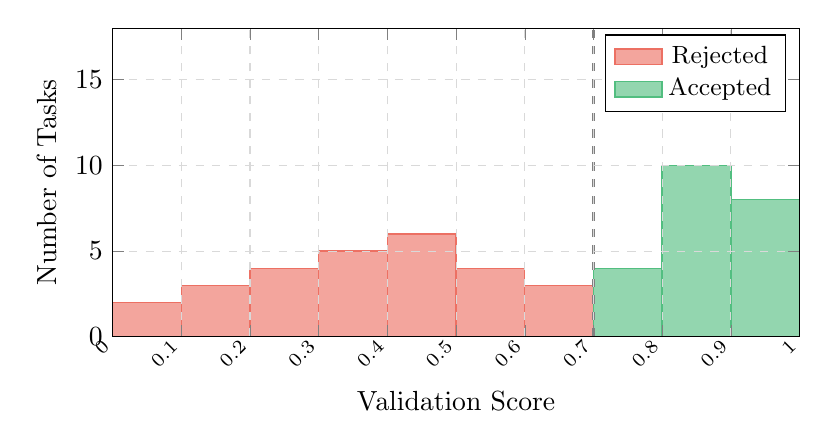
\begin{tikzpicture}
\begin{axis}[
    width=0.85\linewidth,
    height=5.5cm,
    xlabel={Validation Score},
    ylabel={Number of Tasks},
    ymin=0, ymax=18,
    xmin=0, xmax=1.0,
    xtick={0, 0.1, 0.2, 0.3, 0.4, 0.5, 0.6, 0.7, 0.8, 0.9, 1.0},
    xticklabel style={font=\scriptsize, rotate=45, anchor=east},
    grid=major,
    grid style={dashed, gray!30},
    legend style={at={(0.98,0.98)}, anchor=north east, font=\small},
    area style,
]
% Rejected (score < 0.7)
\addplot+[ybar interval, fill=baselinecolor!50, draw=baselinecolor!80, line width=0.5pt]
coordinates {
    (0.0,2) (0.1,3) (0.2,4) (0.3,5) (0.4,6) (0.5,4) (0.6,3)
    (0.7,0)
};
% Accepted (score >= 0.7)
\addplot+[ybar interval, fill=vpercolor!50, draw=vpercolor!80, line width=0.5pt]
coordinates {
    (0.0,0) (0.1,0) (0.2,0) (0.3,0) (0.4,0) (0.5,0) (0.6,0)
    (0.7,4) (0.8,10) (0.9,8) (1.0,0)
};
\draw[dashed, thick, gray] (axis cs:0.7,0) -- (axis cs:0.7,18) node[above, font=\small] {$\tau=0.7$};
\legend{Rejected, Accepted}
\end{axis}
\end{tikzpicture}
\caption{Distribution of validation scores. The dashed line indicates the acceptance threshold $\tau = 0.7$. Tasks scoring below the threshold are rejected and sent back for replanning.}
\label{fig:validator-score}
\end{figure}

\subsection{Error Analysis}

Figure~\ref{fig:error-categories} compares the error category distribution between the baseline and VPER.

\begin{figure}[t]
\centering
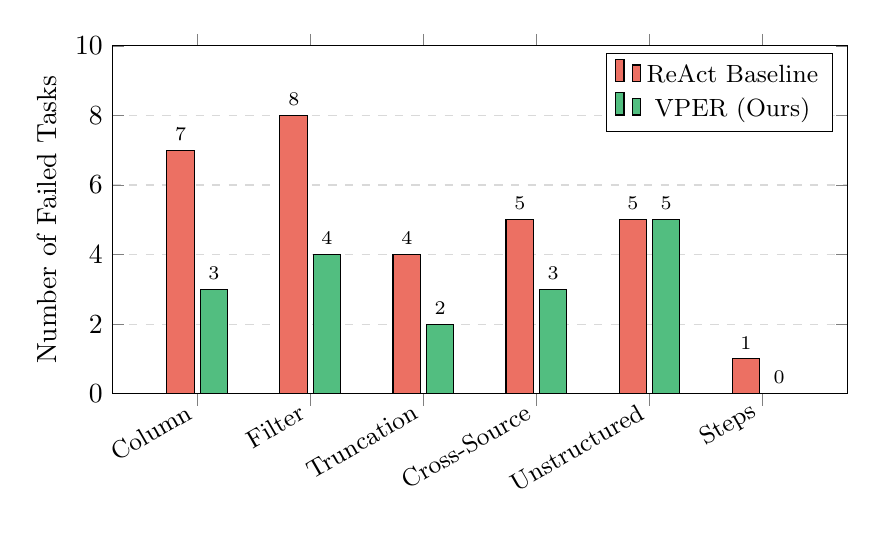
\begin{tikzpicture}
\begin{axis}[
    ybar,
    width=0.9\linewidth,
    height=6cm,
    bar width=10pt,
    ylabel={Number of Failed Tasks},
    symbolic x coords={Column, Filter, Truncation, Cross-Source, Unstructured, Steps},
    xtick=data,
    xticklabel style={font=\small, rotate=30, anchor=east},
    ymin=0, ymax=10,
    legend style={at={(0.98,0.98)}, anchor=north east, font=\small},
    nodes near coords,
    nodes near coords style={font=\scriptsize, above},
    enlarge x limits=0.15,
    grid=major,
    ymajorgrids=true,
    xmajorgrids=false,
    grid style={dashed, gray!30},
]
\addplot[fill=baselinecolor!80] coordinates {
    (Column,7) (Filter,8) (Truncation,4) (Cross-Source,5) (Unstructured,5) (Steps,1)
};
\addplot[fill=vpercolor!80] coordinates {
    (Column,3) (Filter,4) (Truncation,2) (Cross-Source,3) (Unstructured,5) (Steps,0)
};
\legend{ReAct Baseline, VPER (Ours)}
\end{axis}
\end{tikzpicture}
\caption{Error category distribution comparison. VPER reduces errors across most categories, with the largest reductions in column name matching, filter condition errors, and cross-source integration failures. Unstructured document parsing remains an unsolved challenge.}
\label{fig:error-categories}
\end{figure}

VPER reduces errors across most categories:
\begin{itemize}[leftmargin=1.5em]
    \item \textbf{Column name errors} drop from 7 to 3, as the Planner's schema context guides the Executor toward correct column references.
    \item \textbf{Filter condition errors} drop from 8 to 4, as the Replanner can detect and correct failed queries.
    \item \textbf{Cross-source integration errors} drop from 5 to 3, as the Workspace schema map provides a unified view of all data sources.
    \item \textbf{Unstructured data parsing} remains at 5, reflecting the fundamental challenge of extracting structured information from narrative Markdown documents---a limitation that requires dedicated document understanding capabilities beyond VPER's current scope.
\end{itemize}

\subsection{Case Study: Validator-Triggered Correction}

We present a representative case where the Validator successfully identifies and corrects an error.

\textbf{Task 145 (Medium):} ``Among the events attended by more than 10 members of the Student Club, how many of them are meetings?''

\begin{enumerate}[leftmargin=1.5em]
    \item \textbf{Planning:} The Planner generates a 3-step plan: (1) read attendance CSV, (2) query event database schema, (3) join and aggregate with Python.
    \item \textbf{Execution:} The Executor successfully joins attendance and event data, counts attendees per event, filters for $>10$, and identifies 4 meetings.
    \item \textbf{First Validation:} The Validator scores the answer at 0.65 (below threshold 0.7), noting that the trajectory shows redundant schema inspection that could be consolidated.
    \item \textbf{Replanning:} The Replanner adjusts the plan to consolidate schema inspection into the analysis step.
    \item \textbf{Re-execution:} The Executor produces a cleaner result with the correct answer: 4.
    \item \textbf{Second Validation:} The Validator scores 0.82 (above threshold), and the answer is accepted.
\end{enumerate}

This case demonstrates VPER's ability to not only catch incorrect answers but also improve answer quality through iterative validation-replanning cycles.


% ============================================================
\section{Conclusion}
% ============================================================

We presented VPER, a multi-agent framework that augments the Plan-Execute-Replan paradigm with LLM-as-a-Judge answer verification for reliable data analysis.
Through systematic error analysis of the ReAct baseline, we identified three dominant failure modes---myopic execution, lack of replanning, and absence of verification---and addressed each with dedicated modules: a Planner for structured task decomposition, a Replanner for dynamic plan adjustment, and a Validator for pre-submission answer verification.

Experiments on a 50-task benchmark demonstrate that VPER achieves 44.0\% accuracy (69.2\% relative improvement over baseline) while reducing the failure rate from 6.0\% to 2.0\%.
The Validator module alone corrects 10.0\% of incorrectly submitted answers, validating the effectiveness of answer verification before submission.

\paragraph{Limitations and Future Work.}
VPER's current limitations include: (1)~difficulty with unstructured document parsing (all Extreme tasks and many Hard tasks involve narrative Markdown documents); (2)~the Validator introduces additional latency and API costs due to multiple LLM evaluation calls; (3)~the 8.0\% false positive rate of the Validator suggests room for improvement in evaluation precision.
Future work will explore: integrating dedicated document understanding modules, optimizing Validator efficiency through distilled evaluator models, and extending the framework to support multi-turn interactive data analysis.


\bibliographystyle{unsrtnat}
\bibliography{references}

\end{document}
